% https://tex.stackexchange.com/questions/451938/how-to-add-a-label-to-a-vector-and-an-angle

\documentclass[tikz,border=3.14mm]{standalone}
\usepackage{quantikz}
\usetikzlibrary{angles,quotes,arrows.meta}
\begin{document}
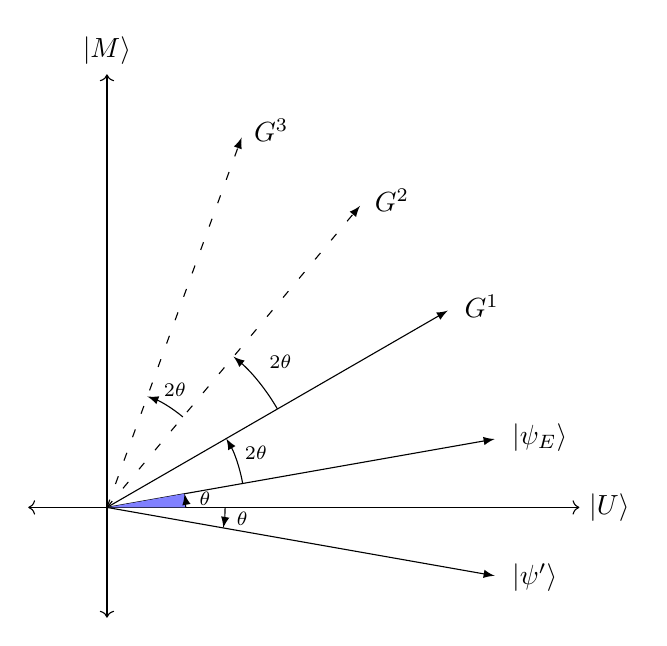
\begin{tikzpicture}[scale=5]
    % X axis
    \draw[<->] (-0.2cm,0cm) -- (1.2cm,0cm) coordinate (U)
      node[right,fill=white] {$\ket{U}$};

    % Y axis
    \draw[<->] (0cm,-0.28cm) -- (0cm,1.10cm) coordinate (M)
      node[above,fill=white] {$\ket{M}$};

    % Equal superposition vector
    \draw[black,-latex]
      (0cm,0cm) coordinate(O) -- (10:1cm) coordinate (pe)
      node[pos=1.02,anchor=west] {$\ket{\psi_E}$};
    %
    \draw pic
      ["\scriptsize{$\theta$}",
       angle eccentricity=1.25,
       draw,
       -latex,
       angle radius=1cm,
       fill=blue!50
      ] 
      {angle = U--O--pe};

    % G(0): reflection about equal U
    \draw[black,-latex]
      (0cm,0cm) coordinate(O) -- (-10:1cm) coordinate (pe1r1)
      node[pos=1.02,anchor=west] {$\ket{\psi'}$};
    %
    \draw pic
    %\draw[<->] pic
      ["\scriptsize{$\theta$}",
       angle eccentricity=1.15,
       draw,
       latex-,
       angle radius=1.5cm,
       %arrows = {-latex[reversed, length=4pt]}
      ] 
      {angle = pe1r1--O--U};

    % G(0): reflection about equal SP
    \draw[black,-latex]
      (0cm,0cm) coordinate(O) -- (30:1cm) coordinate (g1)
      node[pos=1.02,anchor=west]
      {$G^1$};
      %{$\ket{\psi_{1r2}}$};
    %
    \draw pic
    %\draw[<->] pic
      ["\scriptsize{$2\theta$}",
       angle eccentricity=1.15,
       draw,
       -latex,
       angle radius=1.75cm,
       % arrows = {-latex[reversed, length=4pt]}
      ] 
      {angle = pe--O--g1};

    % G2
    \draw[black,loosely dashed,-latex]
      (0cm,0cm) coordinate(O) -- (50:1cm) coordinate (g2)
      node[pos=1.02,anchor=west]
      {$G^2$};
    %
    \draw pic
      ["\scriptsize{$2\theta$}",
       angle eccentricity=1.15,
       draw,
       -latex,
       angle radius=2.5cm,
       % arrows = {-latex[reversed, length=4pt]}
      ] 
      {angle = g1--O--g2};

    % G3
    \draw[black,loosely dashed,-latex]
      (0cm,0cm) coordinate(O) -- (70:1cm) coordinate (g3)
      node[pos=1.02,anchor=west]
      {$G^3$};
    %
    \draw pic
      ["\scriptsize{$2\theta$}",
       angle eccentricity=1.15,
       draw,
       -latex,
       angle radius=1.5cm,
      ] 
      {angle = g2--O--g3};

\end{tikzpicture}
\end{document}
